\chapter{Introduction}\label{chapI}

\section{Introduction générale}

% \subsection{L'intégration de l'environnement sensoriel, une fonction complexe}
De nombreux animaux sont capables de se repérer et de se déplacer dans leur environnement, une fonction complexe qui nécessite de traiter des entrées sensorielles multiples et de produire une réponse motrice adaptée. Le système nerveux, constitué d'un réseau de neurones capables de guider l'information depuis les organes sensoriels vers le cerveau, et depuis le cerveau vers les organes moteurs répond bien à ce problème. Ce traitement centralisé de l'information permet d'atteindre un grand niveau de complexité. On compte par exemple dans le cerveau humain plusieurs dizaines de milliards de neurones.

% \subsection{Des techniques d'imagerie trop locales ou trop globales}
On dispose aujourd'hui d'outils pour appréhender cette complexité comme l'imagerie par résonance magnétique fonctionnelle (IRMf), qui mesure un rapporteur de l'oxygénation du sang, et donc de l'activité locale des tissus cérébraux. Cette technique est cependant limitée à une résolution spatiale de l'ordre du millimètre cube, soit une centaine de milliers de neurones et à une résolution temporelle de l'ordre du Hertz \cite{goense_fmri_2016}. À l'opposé, les techniques d'électrophysiologie comme patch-clamp permettent d'enregistrer l'activité électrique du neurone unique avec une résolution temporelle de l'ordre de la milliseconde mais sont invasives et limitées à une centaine de neurones simultanément \cite{berdondini_active_2009}.

% \subsection{L'échelle intermédiaire, neurones en réseaux sur le cerveau entier}
Ces techniques ont permis beaucoup de découvertes sur le fonctionnement global et local du cerveau, mais peinent à décrire des phénomènes qui concernent l'échelle intermédiaire : un faible nombre de neurones répartis sur l'entièreté du cerveau. C'est précisément à cette échelle que se situe l'intégration multisensorielle, c'est-à-dire la manière dont le cerveau combine l'information liée à plusieurs modalités sensorielles pour produire une représentation cohérente et une réponse motrice unique \cite{stein_multisensory_2008}. Ce phénomène fait appel à la fois aux noyaux sensoriels, à des circuits intégrateurs et aux neurones moteurs, autrement dit une petite centaine de neurones répartis sur le cerveau entier. Pour répondre à ces questions, il a fallu appliquer une nouvelle technique d'imagerie à un nouvel animal modèle.
% VolkerComment
% There are many more neurons implicated especially in the human brain. In the vestibular nucleus almost every neuron responses also to visual stimuli humans ans primats. 

% \subsection{La larve de poisson zèbre, un organisme modèle en neurosciences}
La larve de poisson zèbre, déjà largement utilisée en biologie du développement s'est trouvée bien adaptée à ces questions. Six jours après fertilisation de l’œuf, elle possède déjà un système sensoriel fonctionnel (systèmes visuel, vestibulaire, tactile, auditif...) et un répertoire de comportements riche et complexe (nage, chasse, fuite...). Son cerveau est encore de petite taille (cent mille neurones), mais comporte quasiment toutes les régions anatomiques d'un cerveau de vertébré adulte. On dispose d'une grande variété de lignées notamment des mutants dépigmentés transparents et des lignées transgéniques incluant un rapporteur calcique. Ces lignées permettent une imagerie fonctionnelle par fluorescence pour suivre l'activité des neurones.

% \subsection{La microscopie à feuille de lumière, un scanner 3D rapide}
La technique d'imagerie la plus utilisée en biologie est certainement la microscopie confocale à fluorescence. Il s'agit d'illuminer point par point l'échantillon avec un faisceau laser et de ne collecter que la fluorescence émise par ce point. Cela permet d'atteindre une très bonne résolution spatiale en échange de résolution temporelle. Pour l'imagerie fonctionnelle neuronale du cerveau entier, la microscopie par feuille de lumière est plus adaptée car elle utilise une illumination plan par plan de l'échantillon par une nappe laser. La résolution temporelle est donc largement augmentée tout en conservant une résolution spatiale suffisante, inférieure à la taille d'un neurone. 

% \subsection{La réalité virtuelle pour l'interaction dans un environnement sensoriel riche }
Pour étudier le fonctionnement du cerveau, on fixe donc la larve de poisson zèbre transgénique sous un microscope à feuille de lumière. Il est possible d'étudier l'activité spontanée des neurones, mais pour explorer la réponse du cerveau à une stimulation sensorielle, il faut créer ces stimuli. La manière la plus aboutie de recréer cette stimulation sensorielle est la réalité virtuelle, c'est-à-dire un environnement sensoriel qui réagit aux actions motrices comme si le sujet n'était pas fixé.


\section{Intégration multisensorielle}

\subsection{Définition}

\begin{figure}
  \centering
  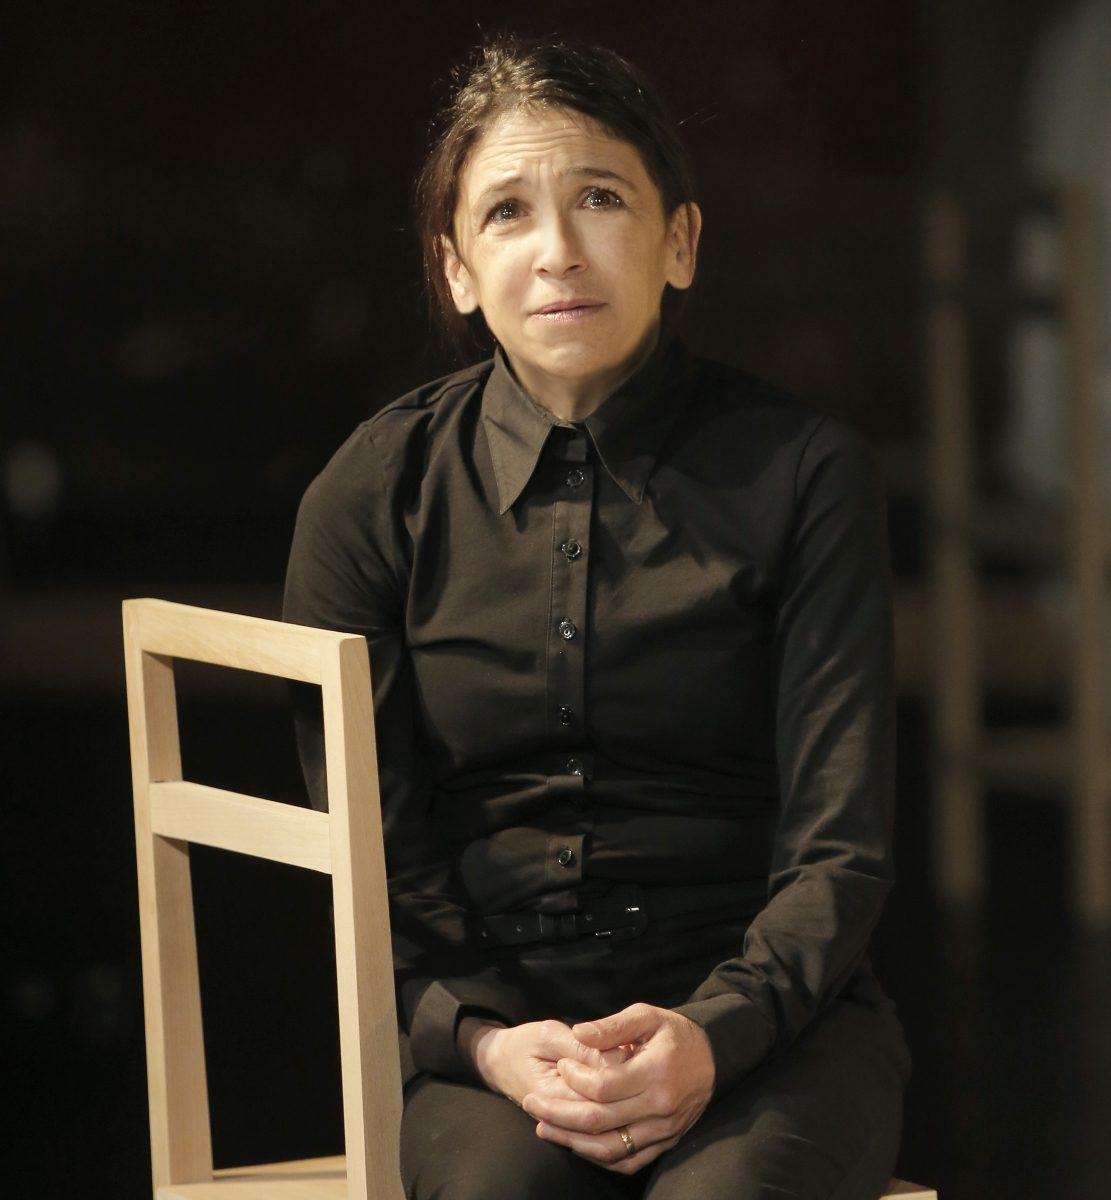
\includegraphics[width=0.5\textwidth]{./files/Kathryn-Hunter_Peter-Brook_valley-of-astonishement.jpg}
  \caption{Kathryn Hunter, dans la pièce de théâtre \emph{The Valley of Astonishment}, mise en scène par Peter Brook. Le personnage est synesthète, et associe dans sa mémoire plusieurs modalités sensorielles.}
  \end{figure}

L'intégration multisensorielle est le processus par lequel le cerveau combine les informations perçues pour produire une représentation interne de l'environnement extérieur. La prise d'information peut passer par plusieurs modalités sensorielles comme les systèmes visuel, vestibulaire, tactile, auditif, olfactif, proprioceptif, ou encore somesthésique. Ces différentes modalités peuvent donner des informations cohérentes qui se complètent pour améliorer la perception mais également des informations contradictoires qui peuvent entrainer des illusions sensorielles.

\subsection{Exemples et illusions}

\subsubsection{Orientation verticale}

Prenons par exemple la perception de l'orientation haut-bas. Le système vestibulaire détecte l'accélération gravitationnelle et nous donne une information de la direction verticale et de l'orientation vers le bas. Le système visuel détecte les lignes verticales dans notre champ de vision (arbres, arêtes des murs) et distingue le ciel lumineux du sol plus sombre. Ces deux modalités sont en général cohérentes, mais on peut concevoir une salle dans lesquelles toutes les lignes sont penchées, ce qui peut perturber nos sens au point de nous faire perdre l'équilibre.

\subsubsection{Reconnaissance du langage}

Autre exemple avec la reconnaissance du langage : on comprend mieux une personne quand on la voit parler. L'information auditive du son de la voix est combinée à l'information visuelle des mouvements des lèvres et autres expressions, ce qui améliore la compréhension. Mais on peut tromper le cerveau en faisant écouter un son qui ne correspond pas au mouvement des lèvres, ce qui est alors interprété comme un autre son (cet effet connu sous le nom McGurk). 

\subsubsection{Détection d'une source sonore}

Le système auditif permet de déterminer approximativement la direction de la source d'un son grâce à l'espacement entre les deux oreilles, information qui peut être confirmée lorsque le système visuel identifie la source. Mais lorsque l'on voit un objet bouger au rythme d'un son provenant d'ailleurs, on peut lui attribuer la source du son et ignorer l'information auditive, c'est l'illusion qu'utilisent les ventriloques pour faire parler leur marionnette \cite{bonath_neural_2007}.

\subsubsection{Illusion proprioceptive}

Un exemple encore plus marquant est l'illusion proprioceptive que l'on peut déclencher avec un casque de réalité virtuelle. Dans une situation normale, le sens du toucher est combiné à l'information visuelle pour déterminer la nature des objets que l'on touche. Mais si l'on présente une main factice en image à un sujet, il peut avoir l'illusion que cette main est la sienne au point de ressentir un objet qui touche la fausse main.

\subsection{Mécanismes et échelles}

Ces multiples exemples montrent l'omniprésence de l'intégration multisensorielle dans les phénomènes perceptifs mais n'en indiquent pas les mécanismes neuronaux. Ces derniers sont complexes, avec une origine à la fois à l'échelle du neurone unique et dans l'organisation du cerveau.

\subsubsection{À l'échelle du cerveau}

Une étude en IRMf chez l'humain s'est intéressée à la structure des zones multisensorielles dans le cerveau \cite{beauchamp_unraveling_2004}. Le sujet était exposé à différents stimuli visuels (des visages) et auditifs (de voix) séparément ou combinés. Alors que les zones unisensorielles sont bien délimitées, les zones multisensorielles se sont révélées très imbriquées.
À l'échelle du cerveau en imagerie fonctionnelle par résonance magnétique, il est difficile de définir un critère sur la nature multisensorielle ou non d'une région. En effet, une étude comparant plusieurs critères statistiques montre que la superadditivité n'est pas toujours un critère pertinent dans l'étude de l'intégration multisensorielle à cette échelle \cite{beauchamp_statistical_2005}.
Alors que l'idée de cortexes sensoriels bien cloisonés était largement adoptée, une étude sur des macaques a montré que des liaisons pouvaient exister entre les différentes aires sensorielles primaires \cite{brosch_nonauditory_2005}. Une autre étude sur la gerbille a montré que le cortex auditif primaire recevait des entrées directes des cortex somatosensoriel, visuel et multisensoriel, ainsi que des structures visuelles et multisensorielles du thalamus et du tronc cérébral \cite{budinger_multisensory_2006}.
Les connexions entre les différentes régions du cerveau sont donc à la base de son fonctionnement multisensoriel. Les différentes aires sensorielles au début considérées comme unimodales se sont révélées multimodales. Les études à cette échelle tendent en effet à montrer que les différentes modalités sensorielles sont fortement liées dès un stade précoce du traitement de l'information \cite{stein_multisensory_2008}.

% The present study has shown, by use of the bidirectional
% and sensitive neuronal tracer FD, that AI of the gerbil
% (1) receives direct inputs from somatosensory, visual, and
% multisensory cortices, as well as from visual and multisen-
% sory thalamic and brainstem structures, and (2) has vari-
% ous projections to somatosensory, olfactory, visual, and
% multisensory cortical and subcortical brain regions.

\subsubsection{À l'échelle du neurone unique}

Les études à l'échelle du cerveau déconstruisent l'idée de grandes régions unisensorielles mais n'excluent pas une ségrégation des différentes modalités sensorielles à l'échelle du neurone. C'est pourquoi des études ont été menées à cette échelle plus locale. Une d'elles a révélé des connexions directes entre des neurones visuel et auditif \cite{bizley_physiological_2007} par électrophysiologie sur des furets. Dans une autre, publiée en 2007 \cite{allman_multisensory_2007}, les auteurs ont enregistré dans le cerveau de chats par électrophysiologie l'activité de milliers de neurones du sillon temporal supérieur en réponse à des stimuli visuels et auditifs combinés. Certains neurones ne répondaient qu'à un seul stimulus (neurone unimodal) alors que d'autre affichaient une réponse dans les deux cas (neurone bimodal). De plus, l'étude montre qu'il existe en proportion égales des neurones ne répondant qu'en présence des deux stimuli simultanés. Ces neurones ne seraient simplement pas détectés dans des expériences qui ne mettant en jeu qu'une seule des modalités sensorielles. À l'échelle du neurone unique, l'intégration multisensorielle se manifeste par des phénomènes tels que la super-additivité ou la sous-additivité. Certains neurones ont une réponse bien plus forte en présence de plusieurs stimuli simultanés que lorsque ceux-ci sont présentés séparément. L'amplitude de ce phénomène est d'autant plus forte que les stimuli présentent une corrélation spatiale et temporelle \cite{stein_multisensory_2008}. 

% Ces phénomènes propres à certains neurones ne sont pas présents dès la naissance et nécessitent une phase d'apprentissage.

\subsubsection{Intégration inconsciente ou interaction}

Dans une revue de 2008 \cite{angelaki_vestibular_2008}, les auteurs présentent le système vestibulaire comme particulièrement adapté à l'exploration de l'intégration multisensorielle. L'intégration multimodale a lieu très tôt dans les réseaux de neurone vestibulaires et il n'y a pas de sensation consciente du signal capté par les organes mais bien une sensation unifiée qui en résulte.
À l'opposé, certain phénomènes d'intégration peuvent avoir lieu de manière consciente, certains auteurs parlent alors d'"interaction multisensorielle" pour distinguer la manière dont plusieurs sensations interagissent entre elles d'une sensation unique résultant de l'intégration \cite{driver_multisensory_2008}. 

% We will often refer to multisensory ‘‘interplay’’ rather than
% the commonly used ‘‘integration,’’ so as to include cases where
% one modality might affect another without necessarily always im-
% plying a single unified percept.

\subsection{Le système vestibulaire chez la larve de poisson zèbre}

\subsubsection{Limites des études actuelles}

Comme nous l'avons vu, le phénomène d'interaction multisensorielle fait intervenir des neurones en petit nombre répartis dans des régions différentes du cerveau. Les études actuelles ont mis en évidence des phénomènes locaux spécifiques à certains neurones et des coactivations de régions globales à différents endroits du cerveau mais ne permettent pas d'obtenir les deux informations en même temps. 
Ces éléments montrent que l'étude de l'intégration multisensorielle doit nécessairement passer par l'analyse des réseaux entiers à l'échelle du neurone unique. Les études en IRM manquent l'échelle du neurone unique et les études d'électrophysiologie manquent les phénomènes de réseau à l'échelle du cerveau entier. C'est pourquoi un nouveau modèle qui permettent de combiner l'échelle du neurone unique et l'échelle du cerveau entier est nécessaire.

\subsubsection{Le poisson zèbre comme animal modèle adapté}

Les cerveaux de mammifères sont composés de milliards de neurones ce qui les rend trop gros pour se prêter à ce genre d'étude. C'est la raison du succès de la larve de poisson zèbre. Ce nouvel animal modèle permet, par la taille réduite de son cerveau et sa transparence de réaliser l'acquisition du cerveau entier à la résolution du neurone par des techniques d'imagerie fonctionnelle \cite{panier_fast_2013}. Cela permet l'étude de phénomènes qui ont lieu à travers tout le cerveau tout en concernant un petit nombre de neurone. Le poisson zèbre partage la structure de son cerveau avec les autres vertébrés tout en ayant un catalogue de comportement assez riche. De nombreuses études concernant ses différentes modalités sensorielles et leur bases neuronales ont été publiées depuis 2013. Comme cité plus haut, le modèle vestibulaire se prête bien à l'étude de l'intégration multisensorielle, c'est donc le système que nous avons choisi d'étudier.


\section[Imagerie fonctionnelle]{Imagerie fonctionnelle par microscopie à feuille de lumière}

% \subsection{Comment enregistrer le cerveau entier ?}
Comme nous l'avons vu, les techniques d'acquisition de l'activité neuronale comme l'électrophysiologie et l'imagerie par résonance magnétique ne sont pas adaptées pour réaliser l'imagerie du cerveau entier à l'échelle du neurone unique. Il est donc nécessaire d'utiliser une technique d'acquisition non invasive capable de telles performances. Travailler sur un animal transparent comme la larve de poisson zèbre facilite l'acquisition utilisant la lumière visible, c'est-à-dire l'imagerie optique. Celle-ci est très développée en biologie et peut assurer à la fois une bonne résolution et un champ large. Cependant, plusieurs innovations importantes à la fois en optique, en ingénierie moléculaire, et en génétique ont dû être combinées pour arriver à un tel résultat. Nous l'introduisons ici.

\subsection{Imagerie fonctionnelle calcique}

\subsubsection{Architecture et fonctionnement du neurone}

\begin{figure}
  \centering
  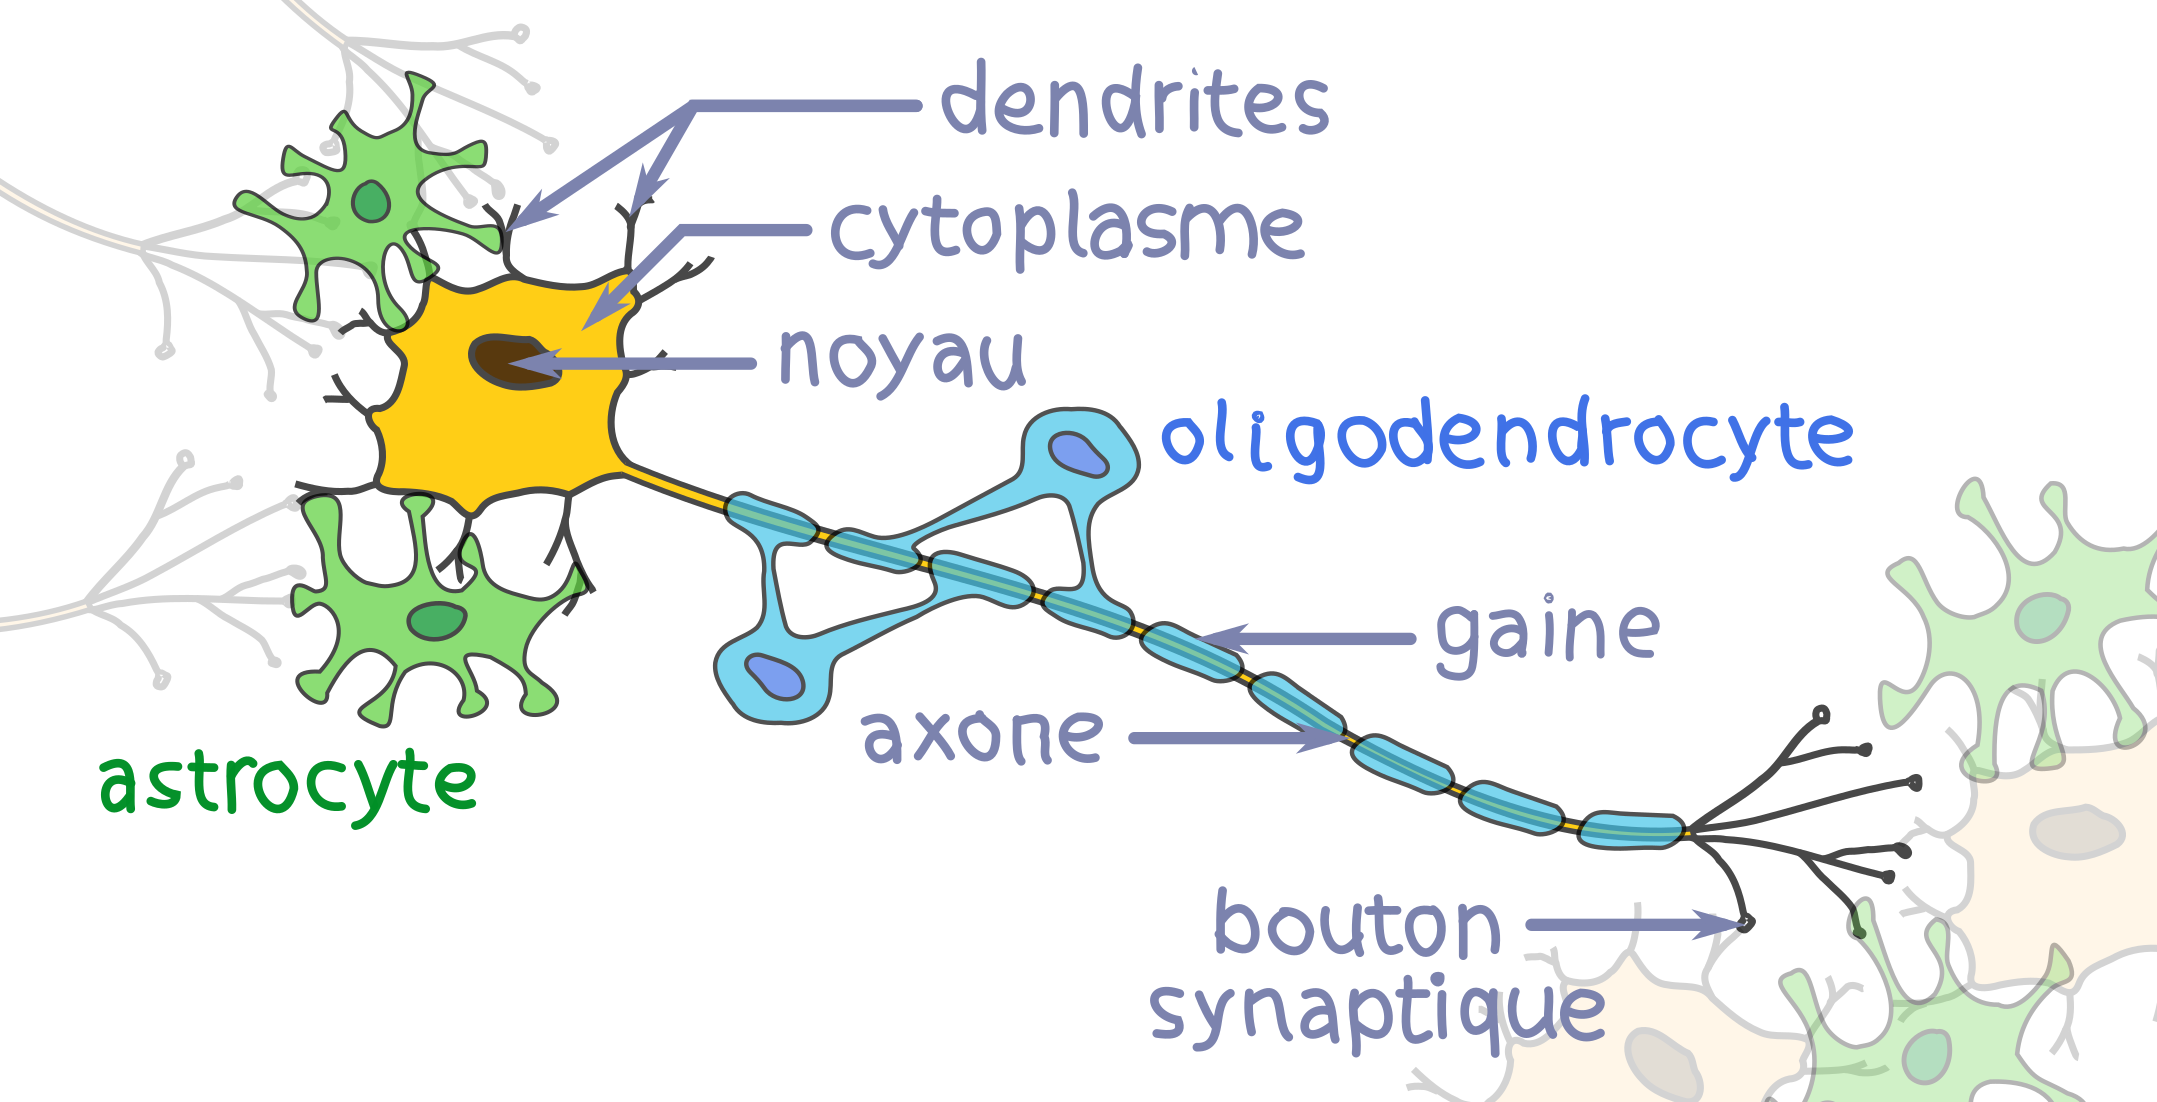
\includegraphics[width=0.8\textwidth]{./files/neurone.svg.png}
  \caption{Schéma d'un neurone accompagné de cellules gliales. Astrocytes (en vert), oligodendrocytes (en bleu). Le neurone dispose d'un long prolongement appelé axone qui le connecte à d'autres neurones via des boutons synaptiques.}
  \end{figure}

Le neurone est une cellule fortement présente dans le cerveau et caractérisée par son prolongement axonal capable de transmettre un influx nerveux. Il est toujours accompagné par des cellules gliales comme les astrocytes ou les oligodendrocytes qui assurent en grande partie les fonctions métaboliques. Il est aujourd'hui considéré comme principal responsable des processus cognitifs bien que de nombreuses recherches montrent l'importance des cellules gliales dans des phénomènes tels que l'intégration du signal calcique et l'établissement de connexions synaptiques \cite{verkhratsky_calcium_1996} \cite{pfrieger_synaptic_1997}.

Le neurone est doté d'une longue projection nommée axone, qui lui permet de se connecter et transmettre un signal à d'autres neurones éloignés de lui. Comme la plupart des cellules, des protéines transmembranaires lui permettent d'atteindre une différence de potentiel avec l'extérieur de -70 mV au repos et comme d'autres cellules dites excitables, cela lui permet de transmettre un signal électrique par ouverture et fermeture de canaux ioniques.

\subsubsection{Le calcium dans le neurone}

\begin{figure}
  \centering
  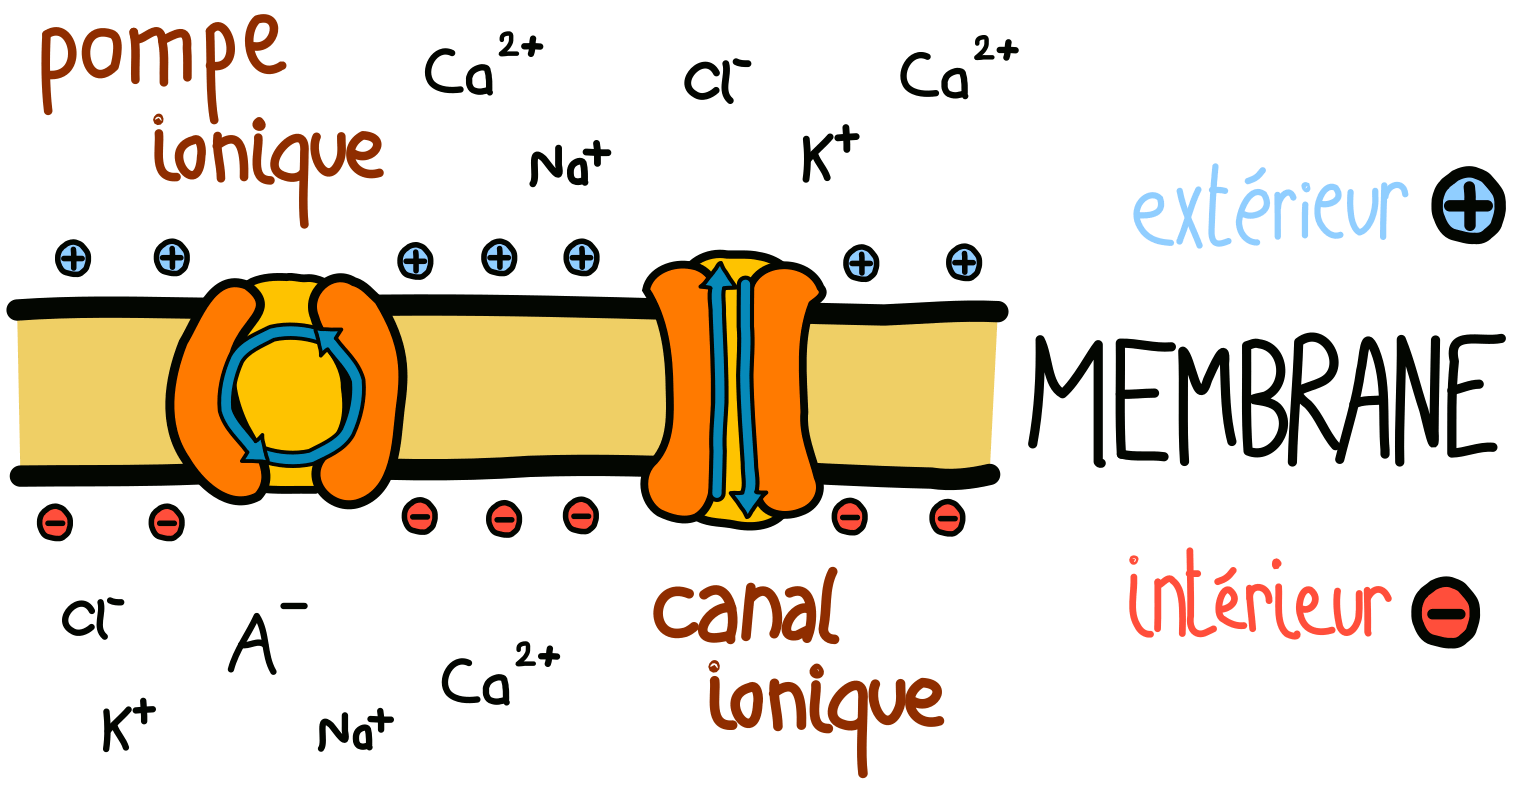
\includegraphics[width=0.8\textwidth]{./files/membrane.svg.png}
  \caption{Des protéines transmembranaires permettent à la cellule de se polariser et de se dépolariser. Les pompes ioniques consomment de l'énergie sous forme d'ATP pour forcer le passage d'ions. Des transporteurs ioniques actifs (symport, antiport) et passifs (uniport) permettent un transport dirigé d'ions. Des canaux sélectifs et non sélectifs permettent un transport rapide.}
  \end{figure}

Le neurone est équipé de pompes et canaux ioniques sur sa membrane qui lui permettent de se polariser en faisant varier la concentration d'ions intracellulaires par rapport au milieu extracellulaire. Ce potentiel électrochimique transmembranaire varie brusquement lors d'événements de dépolarisation qui permettent la propagation d'un message le long des projections axonales vers d'autres neurones. Lors de ces événements, des flux d'ions traversent la paroi cellulaire, ce qui modifie largement leur concentration intracellulaire. Par exemple, l'ion calcium ($Ca^{2+}$) passe d'une concentration de 0.1 µmol/L à 10 µmol/L soit un facteur 100 \cite{grienberger_imaging_2012}, la concentration extracellulaire étant de 1 mmol/L, encore cent fois plus. La durée des potentiels d'actions est de l'ordre de la milliseconde, et la concentration de calcium évolue sur des échelles de temps similaires, de l'ordre de la dizaine de millisecondes. % [?] échelle de temps de la concentration de calcium

\subsubsection{GCaMP, rapporteur calcique}

Du fait de ses grandes variations de concentration, l'ion calcium est un bon indicateur des potentiels d'actions et donc de l'activité neuronale. C'est la raison pour laquelle des rapporteurs calciques ont été développés. Parmi eux, le rapporteur encodé génétiquement GCaMP résulte de l'assemblage entre la calmodulin (calcium modulated protein), une protéine qui se lie au calcium ce qui change sa conformation, et d'une protéine fluorescente verte (GFP, \emph{Green Fluorescent Protein}). Le résultat est une protéine qui devient fluorescente en présence d'ion calcium, avec une dynamique de l'ordre du dixième de seconde. Le code génétique de cette protéine peut être inséré dans une région d'intérêt du génome, pour être exprimée dans des populations ciblées de neurones.

\begin{figure}
\centering
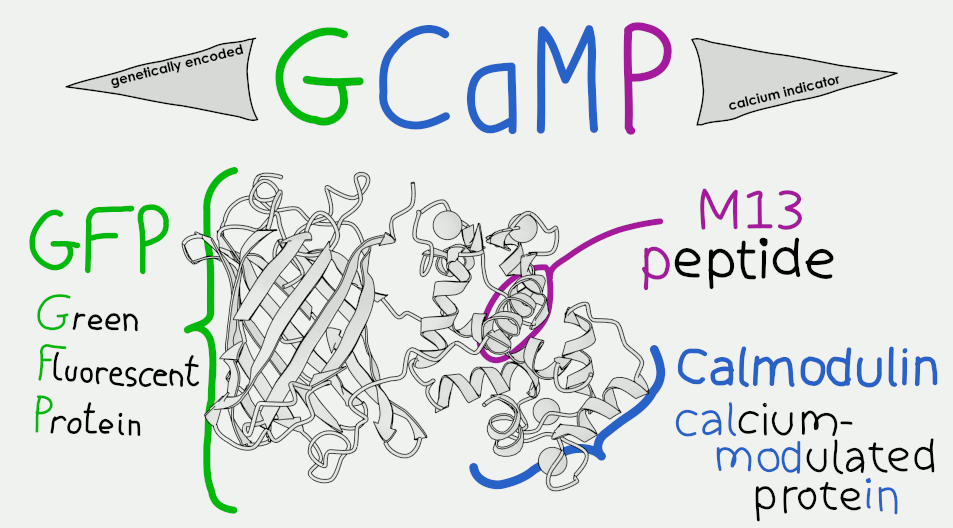
\includegraphics[width=0.8\textwidth]{./files/GCaMP.png}
\caption{Structure tridimensionnelle de l'indicateur calcique GCaMP composée de trois ensembles protéiques.}
\end{figure}

Ainsi, l'organisme génétiquement modifié est équipé d'une molécule présente dans les neurones dont la fluorescence varie en fonction de l'activité du neurone. Cela permet de réaliser l'imagerie fonctionnelle, c'est-à-dire l'imagerie des cellules lors de leur fonctionnement, par l'observation des modifications de leur métabolisme aux échelles de temps courtes. 

\subsection{Microscopie à fluorescence et feuille de lumière}

\subsubsection{Principe de la microscopie}

Le principe général d'un microscope optique est d'éclairer un échantillon et d'observer la lumière qui rentre dans le système de détection. Sur un échantillon mince, on peut faire de la microscopie en transmission ou en réflexion, mais pour un échantillon biologique épais, le phénomène de diffusion rend ces techniques inutilisables. Lorsque le volume imagé est prédéfini, par exemple en imagerie médicale, il faut se contenter de l'auto-fluorescence et élaborer des techniques sophistiqués pour repousser les limites de la diffusion. Au contraire, lorsque l'on contrôle le volume à imager, il est possible de réaliser un marquage fluorescent qui permet de cibler un sous-ensemble précis du tissu biologique et d'émettre autour d'une longueur d'onde choisie.

\subsubsection{Fluorescence}

La fluorescence est un phénomène d’absorption-réémission de lumière par une molécule. Dans le cas de GFP (ainsi que GCaMP), la protéine absorbe les longueurs d'onde dans le bleu et émet dans le vert. Il est ainsi possible de stimuler la fluorescence en utilisant un laser à 488 nm (en imagerie un photon) et de collecter la lumière ré-émise. 

\begin{figure}
\centering
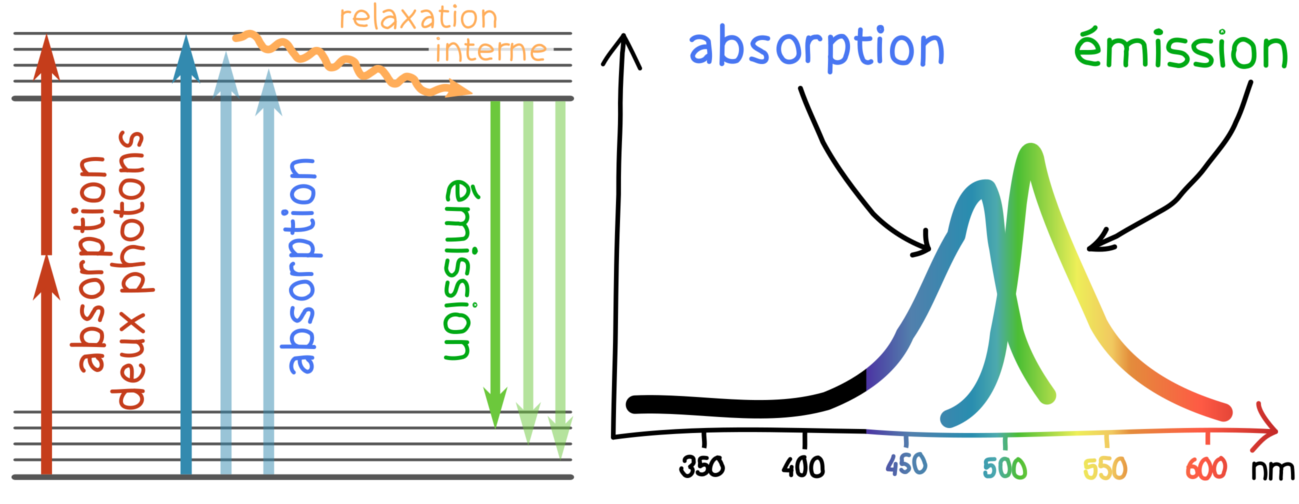
\includegraphics[width=0.8\textwidth]{./files/fluo_couleur.svg.png}
\caption{Illustration du phénomène de fluorescence. À gauche point de vue quantique avec les niveaux d'énergie interne, à droite point de vue ondulatoire avec les spectres d’absorption et d'émission}
\end{figure}

Un des avantages de la microscopie à fluorescence est qu'avec un jeu de filtres adapté, on peut obtenir un excellent rapport signal à bruit. Ainsi, en plaçant sur la ligne de détection un filtre coupe bande à la longueur d'onde du laser, on peut couper toute lumière venant de celui-ci. En ajoutant un filtre passe bande vert, seule la lumière liée à la fluorescence est détectée.

\subsubsection{Sectionnement optique}

Si l'on éclaire l'ensemble d'un échantillon fluorescent et que l'on tente de l'imager avec un objectif de microscope, le rapport signal à bruit est catastrophique. En effet, pour collecter le maximum de lumière, il faut une grande ouverture numérique et donc une faible la profondeur de champ. Un objet lumineux hors du plan focal apparaît donc totalement flou, ce qui constitue une lumière parasite qui couvre celle émise par les objets dans le plan focal. Il faut donc d'une manière ou d'une autre éliminer la lumière provenant d'en dehors du plan focal.

\begin{figure}
  \centering
  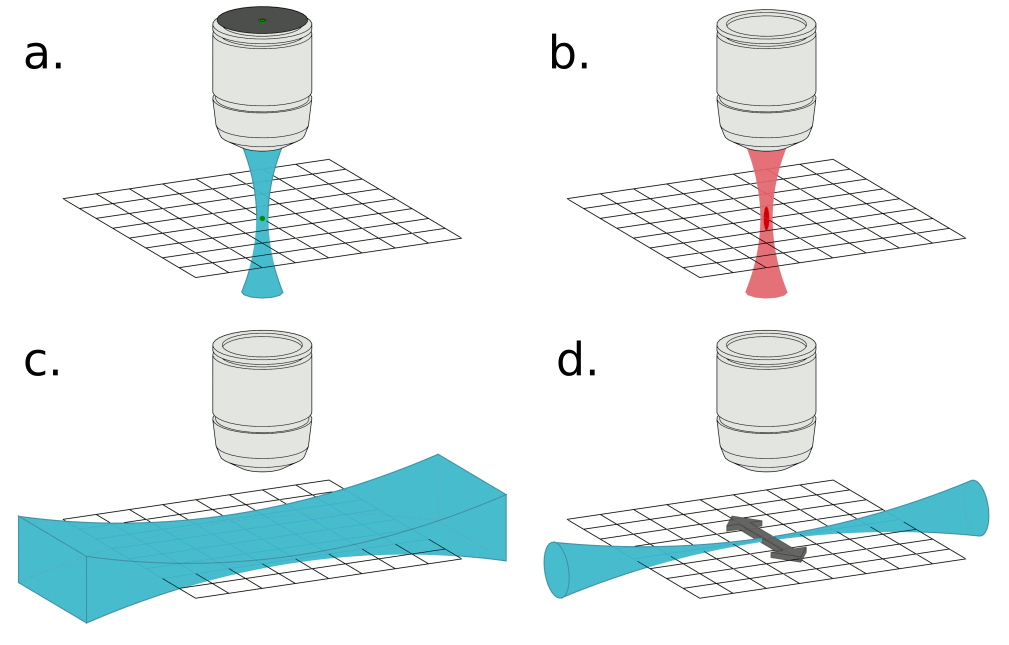
\includegraphics[width=0.8\textwidth]{./files/optical_sectionning.svg.png}
  \caption{Sectionnement optique par différentes techniques \\
  a. Microscopie confocale, un sténopé est placé de manière à bloquer la lumière provenant des points hors focus. \\
  b. Microscopie deux photons, l'effet deux photons permet d'exciter uniquement la fluorescence dans le point de focalisation du laser. \\
  c. Feuille de lumière, une nappe produite avec une lentille cylindrique éclaire une couche de l'échantillon. \\
  d. Balayage laser, une nappe produite par balayage laser éclaire une couche de l'échantillon. \\
  }
  \end{figure}

\subsubsection{Microscopie confocale}

Il existe pour cela plusieurs techniques dites de "sectionnement optique". La plus connue, la microscopie confocale, utilise une illumination focalisée en un seul point. L'objet en ce point est donc fortement éclairé, et le reste beaucoup moins. De plus, un sténopé conjugué à ce point ne laisse passer que la lumière qui en est issue. L'imagerie d'un plan est ensuite obtenue en scannant ce point dans le plan focal, et l'imagerie d'un volume et répétant l'opération pour plusieurs couches. Cette technique est largement répandue et déclinée, et a l'avantage d'être souple et d'atteindre de bonnes résolutions. Cependant, elle ne peut pas combiner une haute définition ($\sim 10^8$ voxels) à une fréquence élevée ($\sim 1$ Hz) et doit sacrifier l'un pour l'autre. Elle est donc réservée soit à l'observation détaillée d'échantillons statiques, soit à l'observation peu détaillée d'échantillons dynamiques. Cette lenteur est liée au fait de scanner un point sur une surface, mais on peut gagner en vitesse au détriment du rapport signal à bruit en éclairant une ligne d'un coup et en remplaçant le trou par une fente, car il suffit alors de scanner dans une seule dimension.

\subsubsection{Microscopie deux photons}

La microscopie deux photons utilise une propriété non linéaire de la lumière pour exciter la fluorescence uniquement en un point. De manière analogue à la microscopie confocale, un faisceau est concentré en un point de l'échantillon, mais l'utilisation d'un laser pulsé dans l'infrarouge permet d'atteindre des niveaux de puissance instantanée bien plus élevés tout en pénétrant mieux les tissus biologiques. De plus, l'utilisation d'un sténopé n'est pas nécessaire car l'effet deux photons est proportionnel au carré de l'intensité lumineuse, et seul le point de focalisation est donc excité. Comme la microscopie confocale, il s'agit alors de scanner un point à travers tout l'échantillon, ce qui est trop lent pour l'imagerie de grands volumes.  

\subsubsection{Microscopie à feuille de lumière}

En microscopie confocale ou deux photons, l'illumination passe par le même objectif que la détection. Mais pour certains échantillons, l'éclairage peut également être fait par le côté. Une feuille de lumière coïncidant avec le plan focal de l'objectif peut être produite à l'aide d'une lentille cylindrique, ou bien par balayage d'un faisceau laser. C'est ce qu'on appelle la microscopie à feuille de lumière, microscopie à nappe laser, ou encore SPIM pour \emph{Single Plane Imaging Microscopy}. Cette technique, en dépit d'un rapport signal à bruit et d'une résolution inférieurs à la microscopie confocale, suffit pour réaliser l'imagerie à la résolution cellulaire. De plus, elle permet d'imager un plan entier d'un seul coup, ce qui est bien pus rapide. En scannant l'objectif et la feuille de lumière, on peut ainsi produire une imagerie volumique à fréquence bien plus élevée qu'en microscopie confocale. Par exemple, avec trente couches espacées de dix microns, on peut acquérir l'ensemble du cerveau d'une larve de poisson zèbre à environ 2Hz.

Si la microscopie par fluorescence à feuille de lumière est une technique particulièrement adaptée à la bio-imagerie fonctionnelle, son utilisation reste toutefois relativement faible. En 2011, un article de revue pointait le manque de système commercial en microscopie à feuille de lumière \cite{santi_light_2011}. En 2017, un autre déplorait le faible niveau de propagation de cette technique au regard de ses performances \cite{power_guide_2017}. La technique reste donc cantonnée à des laboratoires capables de développer leur propre microscope en dépit du succès qu'elle rencontre dans ses applications.



\section[Intégration multisensorielle]{Intégration multisensorielle chez la larve de poisson zèbre}

La microscopie à feuille de lumière permet d'enregistrer le cerveau entier d'une larve de poisson zèbre à la résolution du neurone et avec une fréquence de quelques Hertz. Plusieurs études ont mis en œuvre cette technique pour étudier différents aspects du fonctionnement du cerveau. Je m'intéresse ici aux stratégies mises en œuvre pour étudier l'intégration multisensorielle pour étudier la boucle sensorimotrice, et plus particulièrement sur le modèle visuo-vestibulaire.

% TODO séparer comportement / étude neuronale

\subsection{Boucle sensorimotrice}

Une capacité intéressante du cerveau est le fonctionnement en boucle fermée. En effet, à la manière d'un système d'asservissement, il est capable de mesurer un paramètre extérieur, le comparer à une valeur de commande et agir pour le contrôler. Par exemple, lorsqu'un poisson est emporté par le courant d'une rivière, il détecte un flux optique sous lui et déclenche la nage. Le flux optique résultant est alors la somme de la vitesse du poisson par rapport au fluide et de la vitesse du fluide par rapport au sol. Ce flux optique mesuré permet au poisson d'évaluer si sa nage est efficace pour compenser le courant, s'il doit nager plus vite ou moins vite. Beaucoup des réflexes sont en fait des boucles sensorimotrices dans lesquelles les entrées sensorielles servent en permanence à évaluer la sortie motrice. Deux options se présentent pour étudier ces boucles sensorimotrices. L'une est l'étude en nage libre, l'autre est l'étude en environnement virtuel avec rétroaction.

\subsubsection{Imagerie en nage libre}

Une option pour étudier le poisson dans son environnement naturel est de construire un microscope motorisé capable de suivre les mouvements du poisson lors de la nage de manière à toujours pouvoir imager le cerveau. C'est l'approche adoptée par le laboratoire RoLi \cite{kim_pan-neuronal_2017} qui peut ainsi observer certains comportements difficiles à reproduire avec un poisson immobilisé. L'illumination par le côté étant impossible dans ce cas, c'est une technique de microscopie structurée développée par Jérôme Mertz \cite{mertz_optical_2011} qui a été utilisée.

\subsubsection{Réalité virtuelle}

Une autre option pour étudier la boucle sensorimotrice est de reproduire en environnement virtuel pour simuler la boucle de rétroaction sensorimotrice. Un stimulus sensoriel est soumis au poisson qui réagit en fonction. Sa réponse est mesurée et répercutée sur l'environnement virtuel d'une manière fidèle à la réalité ou volontairement biaisée.

\paragraph{Adaptation motrice fictive}
Ahrens \emph{et al} ont étudié la boucle sensorimotrice dans le cas de l'OMR \cite{ahrens_brain-wide_2012}. Ils ont pour cela créé un environnement fictif dans lequel une larve paralysée est placée au-dessus d'un écran. Des bandes mobiles sont présentées au poisson, ce qui déclenche le réflexe optomoteur. L'activité des neurones moteurs est enregistrée à l'aide d'électrodes (les muscles sont inactifs, car le poisson est paralysé), et ce signal est utilisé pour simuler un déplacement par un mouvement des bandes en sens opposé. Dans cet environnement virtuel, ils ont pu tester des mécanismes comme l'adaptation de gain tout en enregistrant l'activité des neurones. Cela a permis d'identifier les neurones responsables de l'augmentation du gain et de la diminution du gain, qui sont essentiels pour le fonctionnement de la boucle de rétroaction.

\paragraph{Sans rétroaction, comportement d'abandon} % TODO reformuler
Dans le même article \cite{ahrens_brain-wide_2012}, les auteurs ont testé le comportement du poisson dans un système en boucle ouverte, c'est-à-dire sans rétroaction. Les bandes mobiles sont présentées au poisson à vitesse constante sans prendre en compte l'activité des neurones moteurs. Dans cette situation, le comportement de nage est inhibé malgré la présence de stimulus. Cette inhibition due à l'absence de rétroaction peut durer une dizaine de secondes, même après la remise en marche de la rétroaction. Cela montre l'importance du rétrocontrôle dans le fonctionnement de la boucle sensorimotrice et la nécessité d'un système en boucle fermée pour son étude. 

% \paragraph{TODO OKR ?}

% TODO Portugues 2014 Whole-Brain Activity Maps Reveal Stereotyped, Distributed Networks for Visuomotor Behavior

% \paragraph{TODO rhéotaxis ?}

% TODO Oteiza 2017 A novel mechanism for mechanosensory-based rheotaxis in larval zebrafish

% * setups existants pour autres modalités sensorielles
%   * rétroaction système visuel (Portuguese, Ahrens)
% * comment stimuler le système vestibulaire ?
%   * pinces optiques (ne pas parler de pinces magnétiques)
%   * plateforme rotative


\subsection{Modèle viso-vestibulaire}

Un terrain idéal pour étudier l'intégration multisensorielle est le modèle visuo vestibulaire. Ces deux modalités sensorielles sollicitées de concert lors de la nage pour la stabilisation de la posture et de la vision sont pratiquement développées chez la larve de six jours. En effet, le système visuel est fonctionnel dès 4 jours \cite{bollmann_zebrafish_2019}, et le système vestibulaire dès 5 jours (seulement l'utricule) \cite{haddon_early_1996}. Mais avant de décrire les réflexes qui mettent en jeux ces deux modalités sensorielles simultanément, intéressons-nous séparément à l'appareil visuel et à l'appareil vestibulaire.

\subsubsection{Système visuel}

\paragraph{Organisation}
La partie neuronale du système visuel commence par une rétine munie de cellules qui captent la lumière. La répartition des capteurs en fonction de leur couleur correspond aux teintes rencontrées dans l'habitat naturel du poisson. Des circuits neuronaux dans la rétine réalisent un pré-traitement qui, bien qu'en pleine évolution chez une larve de six jours, lui permet déjà de réaliser des opérations complexes. Par exemple, certaines cellules ganglionnaires rétiniennes sont sensibles à l'orientation de motif ou à la direction de mouvement d'un objet, d'autres à la taille d'un objet ou à son évolution \cite{bollmann_zebrafish_2019}. L'étude de l'arborescence de ces ganglions révèle plusieurs zones spécifiques à certains stimuli, comme des variations globales de luminance, le mouvement de petits objets, des déplacements sur tout le champ de vision... La plupart de ces ganglions projettent vers le tectum optique (équivalent du colliculus supérieur chez l'humain) où la suite du traitement est effectuée à travers sa structure laminaire.

\cite{portugues_neural_2009}

\paragraph{OMR, réponse optomotrice}
Certains comportements comme l'OMR (\emph{optomotor response}, réponse optomotrice) et l'OKR (\emph{optokinetic response}, réponse optocinétique) sont purement liés au système visuel. L'OMR est un comportement qui survient de manière très reproductible lors d'un mouvement de translation global dans l'ensemble du champ de vision. La larve se met à nager à l'encontre du flux optique rencontré. Dans la nature, ce comportement permet de compenser le courant d'une rivière pour rester au même niveau en se servant de l'environnement visuel comme référence. En laboratoire, on peut facilement reproduire ce comportement en projetant un motif en translation sous la larve, ce qui provoque des mouvements de queue.

\paragraph{OKR, réponse optocinétique}
L'OKR est un mécanisme de stabilisation de la vision dans lequel l’œil compense les mouvements globaux de l'environnement pour en conserver une vision nette. Cette réponse peut également être étudiée facilement en laboratoire en présentant un motif mobile sur un écran face à une larve. Ces deux comportements sont importants dans l'étude des réponses aux stimulations vestibulaires en présence d'un environnement lumineux. En effet, une accélération ou une rotation de la larve entraîne mécaniquement un mouvement global de l'environnement visuel de celle-ci.

\subsubsection{Système vestibulaire}

\paragraph{Organisation}
L'organe vestibulaire, quant à lui, est situé dans l'oreille interne. Grâce à des cellules ciliées sensibles à leur propre déflexion, il peut mesurer les accélérations inertielle et gravitationnelle auxquelles sont soumises les otolithes (petites pierres osseuses) et les accélérations angulaires du liquide présent dans les canaux semi-circulaires. Bien que quasiment mature chez la larve dès cinq jours, la taille des canaux semi-circulaires les rend inefficaces et donc seule l'utricule (un des otolithes) est fonctionnel. Cela est cependant suffisant (et nécessaire \cite{riley_development_2000}) pour que la larve puisse nager tout en conservant son équilibre.

\begin{figure}
\centering
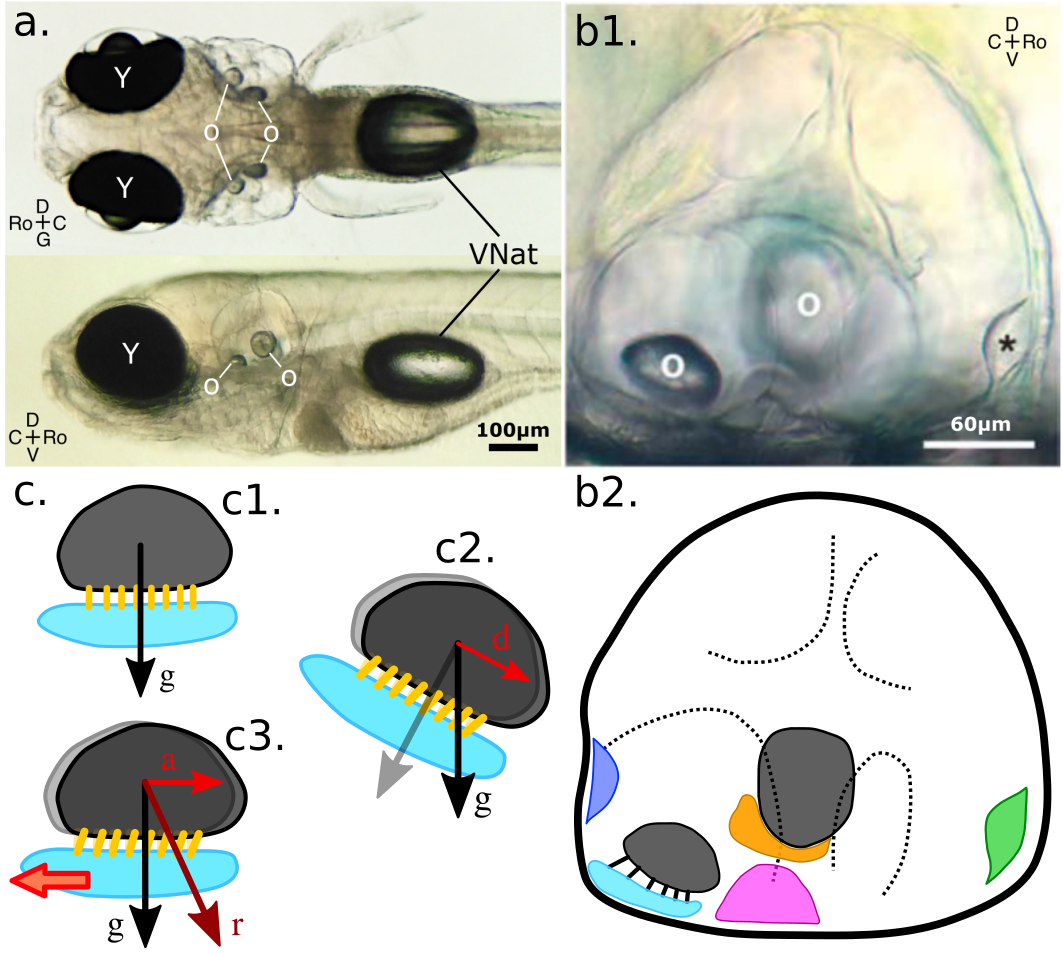
\includegraphics[width=0.6\textwidth]{./files/appareil_vestibulaire.svg.png}
\caption{
Schéma adapté de G. Migault
\\
A. Larve de poisson zèbre de 6 jours vue de dessus (haut) et de côté (bas). On distingue les yeux (Y), l'oreille interne avec ses otolithes (O) et la vessie natatoire (VNat).
\\
B. Agrandissement de l'oreille interne vue de côté (B1) avec le schéma correspondant (B2). On souligne en pointillé les canaux semi-circulaires, en gris les deux otolithes, et en couleur les neuro-épithéliums.
\\
C. Otolithe en fonctionnement. Lorsqu'il est à l'horizontale (C1), les cils sont au repos, lorsqu'il est incliné (C2), les cils sont défléchis car l'accélération gravitationnelle change de direction, lorsqu'il est en mouvement accéléré vers la gauche (C3), l'accélération inertielle (a) s'ajoute à l'accélération gravitationnelle (g) et donne la résultante (r). On voit que l'utricule ne permet pas de différencier l'accélération gravitationnelle de l'accélération inertielle.}
\end{figure}

Les neurones répondant aux stimulations vestibulaires sont présents à de nombreux endroits du cerveau, à la fois dans le prosencéphale (télencéphale, habenulae, thalamus, prétectum), dans le mésencéphale (tectum, nMLF, tegentum), et dans le rombencéphale (cervelet, MON, rhombomère 5-7) \cite{favre-bulle_cellular-resolution_2018}. Chacune de ces régions est impliquée différemment dans les réflexes vestibulaires comme le réflexe vestibulo-oculaire (\emph{vestibulo-ocular reflex}, VOR) et le contrôle postural où réflexe vestibulo-spinal (\emph{vestibulo-spinal reflex}, VSR).

\paragraph{VOR, réflexe vestibulo-oculaire} \label{VOR}
Le VOR, largement répandu chez les vertébrés et également observé chez le poisson-zèbre \cite{bianco_tangential_2012}. C'est un mouvement réflexe des yeux qui compense les mouvements de la tête pour stabiliser la vision. Bianco \emph{et al} l'ont mis en évidence chez la larve de poisson zèbre de plus de 4 jours en la soumettant à une rotation selon l'axe de tangage, ce qui génère une rotation des yeux opposée, avec un angle limité par le maximum physiologique. Le circuit neuronal associé est constitué d'un neurone afférent primaire, un neurone vestibulaire de second ordre, et un motoneurone oculaire qui guide la rotation de l’œil. Ce circuit est présent en deux exemplaires avec une symétrie bilatérale, pour chacun des utricules. Il a également été montré que les neurones du noyau tangentiel ont des projections dans les motoneurones oculaires contra-latéraux, et que ces neurones sont essentiels au fonctionnement du réflexe. 

\paragraph{VSR, réflexe vestibulo-spinal} \label{VSR}
Le VSR est un réflexe de contrôle de posture qui utilise également l'information vestibulaire. Chez le poisson zèbre adulte, la vessie natatoire est un organe important qui permet de contrôler la flottaison, mais chez la larve, elle n'est pas encore fonctionnelle. Les effecteurs du contrôle postural sont donc surtout la queue et les nageoires. Ehrlich \emph{et al} ont étudié le déséquilibre naturel de la larve en \emph{tangage} et ont montré que les événements de nage sont à la base du développement de l'équilibre \cite{ehrlich_control_2017}. Favre-Bulle \emph{et al} ont étudié le contrôle de l'équilibre dans l'axe de \emph{roulis} en stimulant directement les utricules dans l'oreille interne et ont constaté une déflexion proportionnelle de la queue \cite{favre-bulle_cellular-resolution_2018}.

\subsubsection{Intégration viso-vestibulaire}

Les quatre réflexes cités précédemment peuvent être isolés en laboratoire, en contrôlant séparément la stimulation visuelle et la stimulation vestibulaire, mais en réalité, ces réflexes sont très intriqués. En effet, le OKR et le VOR contrôlent tous les deux le mouvement des yeux alors que l'OMR et le VSR contrôlent tous les deux le mouvement de la queue et des nageoires. Dans certains cas, ils peuvent jouer dans le même sens (stimulations cohérentes) alors que dans d'autres ils peuvent entrer en conflit (stimulations incohérentes). C'est précisément cette interaction entre les deux modalités sensorielles qui nous intéresse, et c'est également la raison pour laquelle le système vestibulo-oculaire se prête particulièrement bien à l'étude des stimulations multimodales. Une première étude montre comment dans certains cas, l'information visuelle peut moduler les rotations de l'œil induites par l'utricule \cite{bianco_tangential_2012}.


\section{Objectifs de la thèse}

% TODO Volker (objectifs thèse)
% Open question. Hypotheses. Outline your personal thesis work and results

Les objectifs de ma thèse ont été d'une part de reproduire la boucle sensorimotrice du contrôle postural dans un environnement virtuel, et d'autre part de réaliser un montage capable d'acquérir l'activité neuronale lors de stimulations visuelle et vestibulaire simultanées.